\subsubsection{Package sequenziatore.client.view.process_owner}
\subsubsection{Package sequenziatore::client::iview::iprocessowner}

\paragraph{IMainProcessOwner}
\begin{figure}[H] \centering 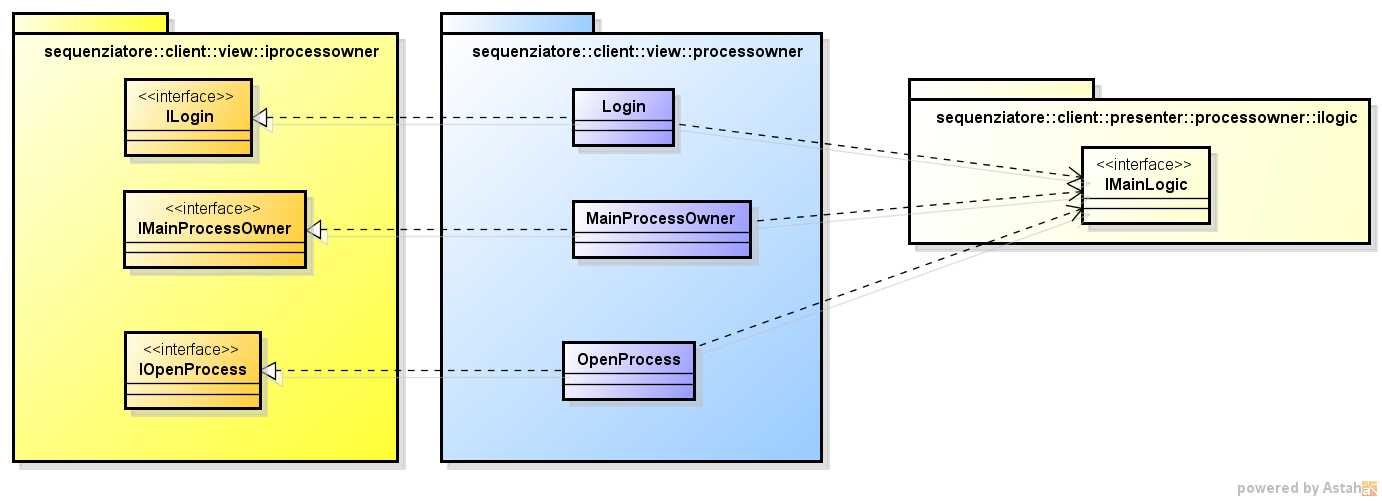
\includegraphics[width=%
\textwidth]
{./pack/ProcessOwner.png} \caption{Diagramma view principale process owner}
\end{figure}
\begin{itemize}
\item \textbf{Nome:} \texttt{IMainProcessOwner};
\item \textbf{Package:} \texttt{\iViewAdmin{}};
\item \textbf{Descrizione:} Interfaccia che permette la gestione delle principali componenti dell'interfaccia grafica dell'utente \textit{process owner\ped{G}}.
\end{itemize}

\paragraph{IUpdateView}
\begin{figure}[H] \centering 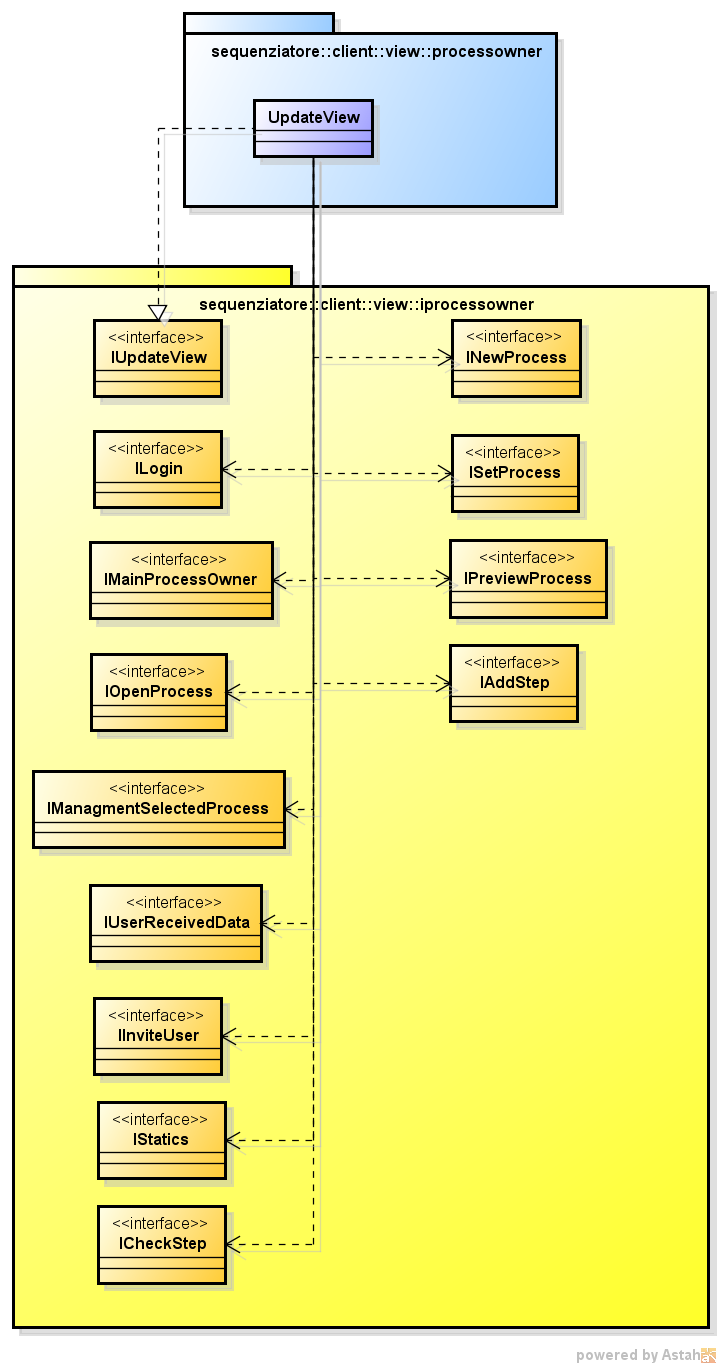
\includegraphics[scale=0.5]
{./pack/UpdateViewPo.png} \caption{Diagramma aggiornamento view process owner}
\end{figure}
\begin{itemize}
\item \textbf{Nome:} \texttt{IUpdateView};
\item \textbf{Package:} \texttt{\iViewAdmin{}};
\item \textbf{Descrizione:} Interfaccia che permette di gestire l'aggiornamento dei \textit{widget\ped{G}} della componente \textit{view}.
\end{itemize}

\paragraph{ILogin}
\begin{itemize}
\item \textbf{Nome:} \texttt{ILogin};
\item \textbf{Package:} \texttt{\iViewAdmin{}};
\item \textbf{Descrizione:} Interfaccia che permette di gestire l'interfaccia grafica relativa alle richieste di autenticazione e chiusura della sessione da parte dell'utente \textit{process owner\ped{G}}.
\end{itemize}

\paragraph{ISetProcess}
\begin{figure}[H] \centering 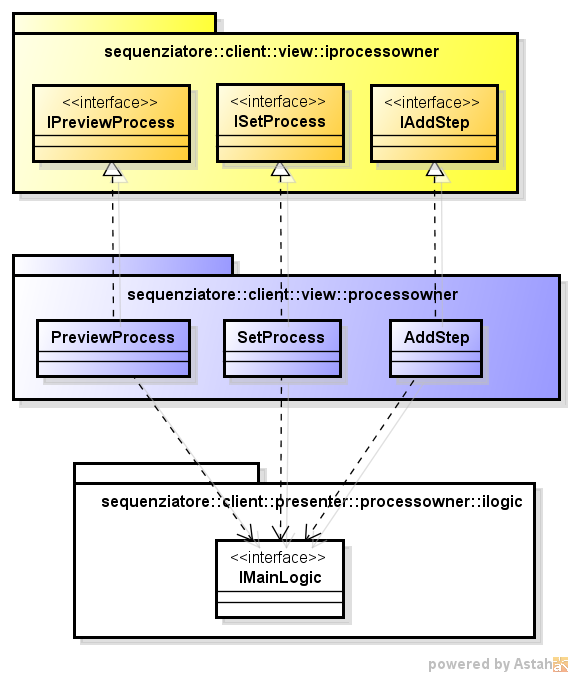
\includegraphics[width=%
\textwidth]
{./pack/newProcess.png} \caption{Diagramma view creazione nuovo processo}
\end{figure}
\begin{itemize}
\item \textbf{Nome:} \texttt{ISetProcess};
\item \textbf{Package:} \texttt{\iViewAdmin{}};
\item \textbf{Descrizione:} Interfaccia che permette di gestire l'interfaccia grafica che consente di creare nuovi processi.
\end{itemize}

\paragraph{IAddStep}
\begin{itemize}
\item \textbf{Nome:} \texttt{IAddStep};
\item \textbf{Package:} \texttt{\iViewAdmin{}};
\item \textbf{Descrizione:} Interfaccia che permette di gestire l'interfaccia grafica che consente di definire un nuovo passo del processo in creazione.
\end{itemize}

\paragraph{IPreviewProcess}
\begin{itemize}
\item \textbf{Nome:} \texttt{IPreviewProcess};
\item \textbf{Package:} \texttt{\iViewAdmin{}};
\item \textbf{Descrizione:} Interfaccia che permette realizzare i \textit{widget} che consentono di visualizzare l'anteprima del processo in creazione.
\end{itemize}

\paragraph{IOpenProcess}
\begin{itemize}
\item \textbf{Nome:} \texttt{IOpenProcess};
\item \textbf{Package:} \texttt{\iViewAdmin{}};
\item \textbf{Descrizione:} Interfaccia che permette di realizzare i \textit{widget} che consentono di aprire un processo tramite ricerca o selezione da una lista.
\end{itemize}

\paragraph{IManagmentSelectedProcess}
\begin{figure}[H] \centering 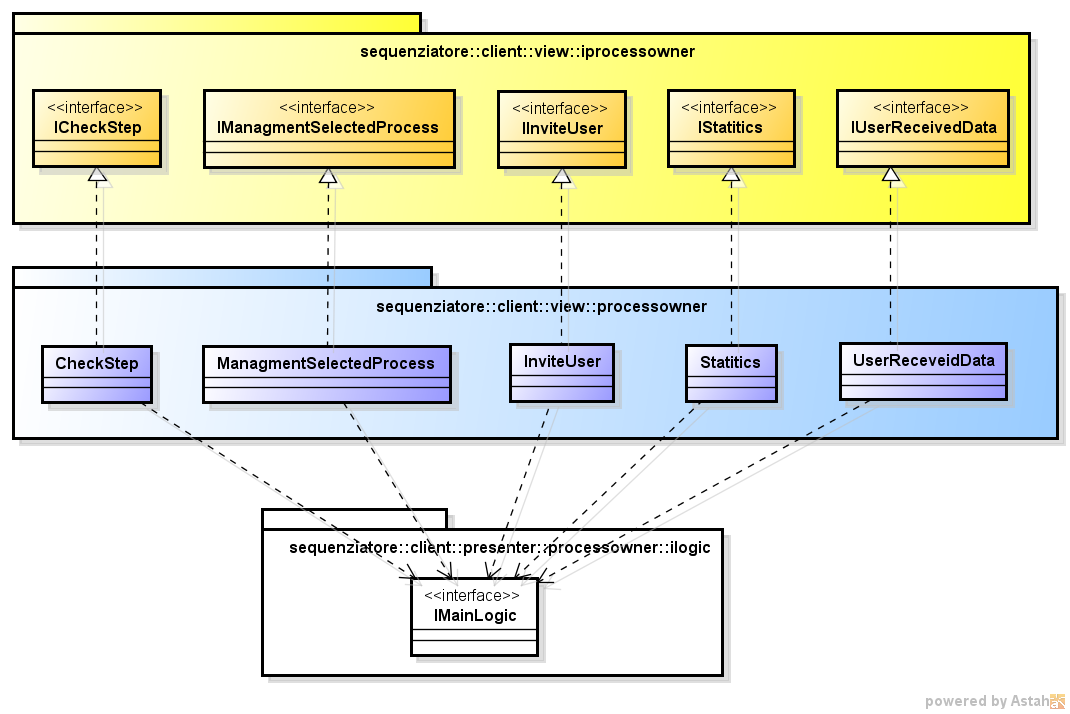
\includegraphics[width=%
\textwidth]
{./pack/PO_ManagmentSelectedProcess.png} \caption{Diagramma view gestione processi creati}
\end{figure}
\begin{itemize}
\item \textbf{Nome:} \texttt{IManagmentSelectedProcess};
\item \textbf{Package:} \texttt{\iViewAdmin{}};
\item \textbf{Descrizione:} Interfaccia che permette di realizzare i \textit{widget} che consentono di gestire i processi selezionati.
\end{itemize}

\paragraph{ICheckStep}
\begin{itemize}
\item \textbf{Nome:} \texttt{ICheckStep};
\item \textbf{Package:} \texttt{\iViewAdmin{}};
\item \textbf{Descrizione:} Interfaccia che permette di realizzare i \textit{widget} che consentono di gestire il controllo dei passi che richiedono intervento umano.
\end{itemize}

\paragraph{IStatistics}
\begin{itemize}
\item \textbf{Nome:} \texttt{IStatistics};
\item \textbf{Package:} \texttt{\iViewAdmin{}};
\item \textbf{Descrizione:} Interfaccia che permette di realizzare i \textit{widget} che consentono di gestire l'accesso alle informazioni statistiche sui processi.
\end{itemize}

\paragraph{IUserReceivedData}
\begin{itemize}
\item \textbf{Nome:} \texttt{IUserReceivedData};
\item \textbf{Package:} \texttt{\iViewAdmin{}};
\item \textbf{Descrizione:} Classe che permette di realizzare i \textit{widget} che consentono di gestire l'accesso ai dati inviati al \textit{server\ped{G}} dagli utenti;
\end{itemize}

\paragraph{IInviteUser}
\begin{itemize}
\item \textbf{Nome:} \texttt{IInviteUser};
\item \textbf{Package:} \texttt{\iViewAdmin{}};
\item \textbf{Descrizione:} Interfaccia che permette di realizzare i \textit{widget} che consentono di gestire i permessi di iscrizione ad un processo da parte degli utenti.
\end{itemize}
\paragraph{MainProcessOwner}
\begin{flushleft}
\begin{itemize}
\item \textbf{Nome:} \texttt{MainProcessOwner};
\item \textbf{Package:} \texttt{\viewAdmin{}};
\item \textbf{Descrizione:} Classe che permette la gestione delle principali componenti dell'interfaccia grafica dell'utente \textit{process owner\ped{G}};
\item \textbf{Relazioni con altri componenti:}
\begin{sloppypar}
La classe implementa l'interfaccia \texttt{\iViewAdmin{}::I\fshyp{}Main\fshyp{}Pro\fshyp{}cess\fshyp{}Ow\fshyp{}ner} e comunica con il \textit{presenter} utilizzando metodi della classe \texttt{\logicAdmin{}::Main\fshyp{}Lo\fshyp{}gic}.
\end{sloppypar}
\end{itemize}
\end{flushleft}

\paragraph{UpdateView}
\begin{flushleft}
\begin{itemize}
\item \textbf{Nome:} \texttt{UpdateView};
\item \textbf{Package:} \texttt{\viewAdmin{}};
\item \textbf{Descrizione:} Classe che permette di gestire l'aggiornamento dei \textit{widget\ped{G}} della componente \textit{view};
\item \textbf{Relazioni con altri componenti:}
\begin{sloppypar}
La classe implementa l'interfaccia \texttt{\iViewAdmin{}::I\fshyp{}Up\fshyp{}da\fshyp{}te\fshyp{}View} e aggiorna le componenti della \textit{view} comunicando con le seguenti classi:
\begin{itemize}
\item \texttt{\viewUser{}::MainProcessOwner};
\item \texttt{\viewUser{}::Login};
\item \texttt{\viewUser{}::SetProcess};
\item \texttt{\viewUser{}::AddStep};
\item \texttt{\viewUser{}::PreviewProcess};
\item \texttt{\viewUser{}::OpenProcess};
\item \texttt{\viewUser{}::ManagmentSelectedProcess};
\item \texttt{\viewUser{}::CheckStep};
\item \texttt{\viewUser{}::UserReceivedData};
\item \texttt{\viewUser{}::Statistics};
\item \texttt{\viewUser{}::InviteUser}.
\end{itemize}
\end{sloppypar}
\end{itemize}
\end{flushleft}

\paragraph{Login}
\begin{flushleft}
\begin{itemize}
\item \textbf{Nome:} \texttt{Login};
\item \textbf{Package:} \texttt{\viewAdmin{}};
\item \textbf{Descrizione:} Classe che permette di gestire l'interfaccia grafica relativa alle richieste di autenticazione e chiusura della sessione da parte dell'utente \textit{process owner\ped{G}};
\item \textbf{Relazioni con altri componenti:}
\begin{sloppypar}
La classe implementa l'interfaccia \texttt{\iViewAdmin{}::I\fshyp{}Lo\fshyp{}gin} e comunica con il\textit{presenter} utilizzando metodi della classe \texttt{\logicAdmin{}::Main\fshyp{}Lo\fshyp{}gic}.
\end{sloppypar}
\end{itemize}
\end{flushleft}

\paragraph{SetProcess}
\begin{flushleft}
\begin{itemize}
\item \textbf{Nome:} \texttt{SetProcess};
\item \textbf{Package:} \texttt{\viewAdmin{}};
\item \textbf{Descrizione:} Classe che permette di gestire l'interfaccia grafica che consente di creare nuovi processi;
\item \textbf{Relazioni con altri componenti:}
\begin{sloppypar}
La classe implementa l'interfCheckStepaccia \texttt{\iViewAdmin{}::I\fshyp{}Set\fshyp{}Pro\fshyp{}cess} e comunica con il\textit{presenter} utilizzando metodi della classe \texttt{\logicAdmin{}::Main\fshyp{}Lo\fshyp{}gic}.
\end{sloppypar}
\end{itemize}
\end{flushleft}

\paragraph{AddStep}
\begin{flushleft}
\begin{itemize}
\item \textbf{Nome:} \texttt{AddStep};
\item \textbf{Package:} \texttt{\viewAdmin{}};
\item \textbf{Descrizione:} Classe che permette di gestire l'interfaccia grafica che consente di definire un nuovo passo del processo in creazione;
\item \textbf{Relazioni con altri componenti:}
\begin{sloppypar}
La classe implementa l'interfaccia \texttt{\iViewAdmin{}::I\fshyp{}Add\fshyp{}Step} e comunica con il\textit{presenter} utilizzando metodi della classe \texttt{\logicAdmin{}::Main\fshyp{}Lo\fshyp{}gic}.
\end{sloppypar}
\end{itemize}
\end{flushleft}

\paragraph{PreviewProcess}
\begin{flushleft}
\begin{itemize}
\item \textbf{Nome:} \texttt{PreviewProcess};
\item \textbf{Package:} \texttt{\viewAdmin{}};
\item \textbf{Descrizione:} Classe che permette realizzare i\textit{widget} che consentono di visualizzare l'anteprima del processo in creazione;
\item \textbf{Relazioni con altri componenti:}
\begin{sloppypar}
La classe implementa l'interfaccia \texttt{\iViewAdmin{}::I\fshyp{}Pre\fshyp{}view\fshyp{}Pro\fshyp{}cess} e comunica con il\textit{presenter} utilizzando metodi della classe \texttt{\logicAdmin{}::Main\fshyp{}Lo\fshyp{}gic}.
\end{sloppypar}
\end{itemize}
\end{flushleft}

\paragraph{OpenProcess}
\begin{flushleft}
\begin{itemize}
\item \textbf{Nome:} \texttt{OpenProcess};
\item \textbf{Package:} \texttt{\viewAdmin{}};
\item \textbf{Descrizione:} Classe che permette di realizzare i\textit{widget} che consentono di aprire un processo tramite ricerca o selezionandolo da una lista;
\item \textbf{Relazioni con altri componenti:}
\begin{sloppypar}
La classe implementa l'interfaccia \texttt{\iViewAdmin{}::I\fshyp{}O\fshyp{}pen\fshyp{}Pro\fshyp{}cess} e comunica con il\textit{presenter} utilizzando metodi della classe \texttt{\logicAdmin{}::Main\fshyp{}Lo\fshyp{}gic}.
\end{sloppypar}
\end{itemize}
\end{flushleft}

\paragraph{ManagmentSelectedProcess}
\begin{flushleft}
\begin{itemize}
\item \textbf{Nome:} \texttt{ManagmentSelectedProcess};
\item \textbf{Package:} \texttt{\viewAdmin{}};
\item \textbf{Descrizione:} Classe che permette di realizzare i\textit{widget} che consentono di gestire i processi selezionati;
\item \textbf{Relazioni con altri componenti:}
\begin{sloppypar}
La classe implementa l'interfaccia \texttt{\iViewAdmin{}::I\fshyp{}Ma\fshyp{}na\fshyp{}gment\fshyp{}Se\fshyp{}lec\fshyp{}ted\fshyp{}Pro\fshyp{}cess} e comunica con il\textit{presenter} utilizzando metodi della classe \texttt{\logicAdmin{}::Main\fshyp{}Lo\fshyp{}gic}.
\end{sloppypar}
\end{itemize}
\end{flushleft}

\paragraph{CheckStep}
\begin{flushleft}
\begin{itemize}
\item \textbf{Nome:} \texttt{CheckStep};
\item \textbf{Package:} \texttt{\viewAdmin{}};
\item \textbf{Descrizione:} Classe che permette di realizzare i\textit{widget} che consentono di gestire l'approvazione dei passi che richiedono intervento umano;
\item \textbf{Relazioni con altri componenti:}
\begin{sloppypar}
La classe implementa l'interfaccia \texttt{\iViewAdmin{}::I\fshyp{}Check\fshyp{}Step} e comunica con il\textit{presenter} utilizzando metodi della classe \texttt{\logicAdmin{}::Main\fshyp{}Lo\fshyp{}gic}.
\end{sloppypar}
\end{itemize}
\end{flushleft}

\paragraph{UserReceivedData}
\begin{flushleft}
\begin{itemize}
\item \textbf{Nome:} \texttt{UserReceivedData};
\item \textbf{Package:} \texttt{\viewAdmin{}};
\item \textbf{Descrizione:} Classe che permette di realizzare i\textit{widget} che consentono di gestire l'accesso ai dati inviati al\textit{server\ped{G}} dagli utenti;
\item \textbf{Relazioni con altri componenti:}
\begin{sloppypar}
La classe implementa l'interfaccia \texttt{\iViewAdmin{}::I\fshyp{}U\fshyp{}ser\fshyp{}Re\fshyp{}cei\fshyp{}ved\fshyp{}Da\fshyp{}ta} e comunica con il\textit{presenter} utilizzando metodi della classe \texttt{\logicAdmin{}::Main\fshyp{}Lo\fshyp{}gic}.
\end{sloppypar}
\end{itemize}
\end{flushleft}

\paragraph{Statistics}
\begin{flushleft}
\begin{itemize}
\item \textbf{Nome:} \texttt{Statistics};
\item \textbf{Package:} \texttt{\viewAdmin{}};
\item \textbf{Descrizione:} Classe che permette di realizzare i\textit{widget} che consentono di gestire l'accesso alle informazioni statistiche sui processi;
\item \textbf{Relazioni con altri componenti:}
\begin{sloppypar}
La classe implementa l'interfaccia \texttt{\iViewAdmin{}::I\fshyp{}Sta\fshyp{}tis\fshyp{}tics} e comunica con il\textit{presenter} utilizzando metodi della classe \texttt{\logicAdmin{}::Main\fshyp{}Lo\fshyp{}gic}.
\end{sloppypar}
\end{itemize}
\end{flushleft}

\paragraph{InviteUser}
\begin{flushleft}
\begin{itemize}
\item \textbf{Nome:} \texttt{InviteUser};
\item \textbf{Package:} \texttt{\viewAdmin{}};
\item \textbf{Descrizione:} Classe che permette di realizzare i\textit{widget} che consentono di gestire i permessi di iscrizione ad un processo da parte degli utenti;
\item \textbf{Relazioni con altri componenti:}
\begin{sloppypar}
La classe implementa l'interfaccia \texttt{\iViewAdmin{}::I\fshyp{}In\fshyp{}vi\fshyp{}te\fshyp{}U\fshyp{}ser} e comunica con il\textit{presenter} utilizzando metodi della classe \texttt{\logicAdmin{}::Main\fshyp{}Lo\fshyp{}gic}.
\end{sloppypar}
\end{itemize}
\end{flushleft}